%!TEX root = main.tex

\section{Datasets}
\label{sec:dataset}

\subsection{Data description}
\label{sub:data-des}
The four TCP connections of the front-end server use different port number to distinguish each other. We use tcpdump to collect the TCP traces of all the four connections in one front-end relay server. Our collection span from July 15, 2015 to July 22, 2015, totally 7 days, 24 hours each day. 

Figure~\ref{fig:use-fre} shows the users' upload and download times over one week. In the figure, we can observe that number of download flows is much higher than the number of upload flows, which means that more users watch video instead of sharing their videos. For both upload and download flows, they continue to grow after 6 a.m. and at about 11 p.m. they reach the peak. Consumers watch or share the crowdsourced live video more often in the night. And the peak of the whole week is at Saturday midnight. It is easy to understand as most people use the crowdsourced live video as a kind of entertainment and do not use it in work time. 

\begin{figure}[t]
\centering
\subfloat[Number of users' upload and download flows.]{
	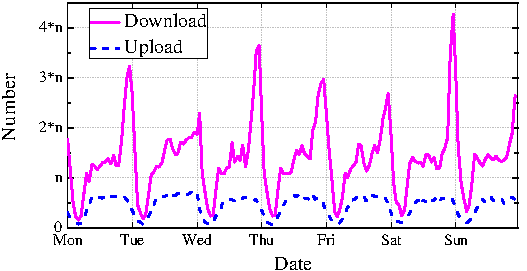
\includegraphics[width=2.5in]{use-fre}
	\label{fig:use-fre}}
\hspace{1em}%
\subfloat[Upload and download flows' complete time.]{
	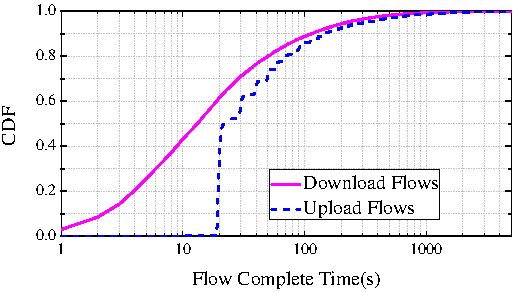
\includegraphics[width=2.5in]{flow-time}
	\label{fig:flow-time}}
	\hspace{1em}%
\subfloat[Upload and download flows' size.]{
	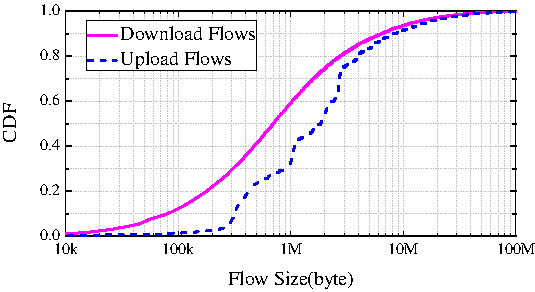
\includegraphics[width=2.5in]{flow-size}
	\label{fig:flow-size}}
\subfloat[The rate of upload and download flow.]{
	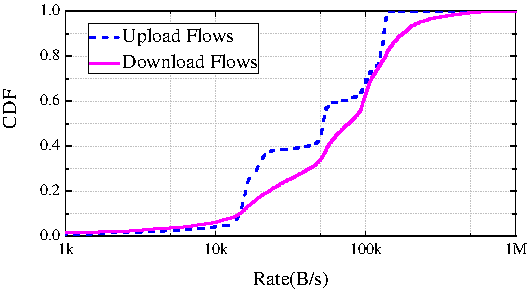
\includegraphics[width=2.5in]{rate}
	\label{fig:flow-rate}}
\caption{Dataset  description.}%
\label{fig:dataset} %% label for entire figure
\termspace
\end{figure}


\iffalse
\begin{figure}[ht]
	\centering
	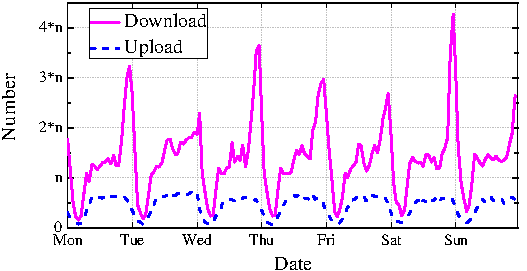
\includegraphics[width=\linewidth]{use-fre}
	\caption{Number of users' upload and download flows.}
	\label{fig:use-fre}
	\termspace
\end{figure}
\fi

Figure~\ref{fig:flow-time} shows the upload and download flows' flow complete time. For download flows, we define the flow complete time as the interval that the front-end server receives the first SYN packet until it receives the acknowledgment of the last packet. For upload flows, the flow complete time is defined as the interval that the front-end server receives the first SYN packet until it receives the last packet from the client. For upload flows, the servers will send keep-alive packet to keep the flow alive and will terminate the flows if it can not receive any frame from client until 20s. That is why there are almost not upload flows which are less than 20s. For both upload and download flows, about 60\% flows are less than 30s. That means most consumers watch or share short videos. As some viewers may terminate to watch the video while the video providers may continue to upload video, the flow complete time of upload flows are longer than download flows.   

%\begin{figure}[ht]
%	\centering
%	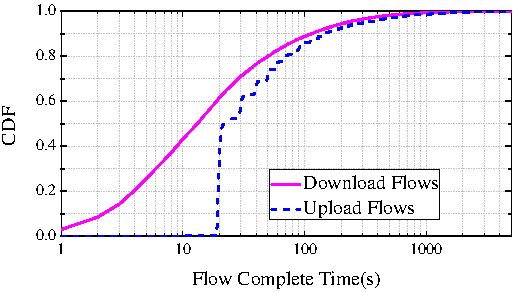
\includegraphics[width=\linewidth]{flow-time}
%	\caption{Upload and download flow complete time.}
%	\label{fig:flow-time}
%	\termspace
%\end{figure}

Figure~\ref{fig:flow-size} shows the upload and download flows' size. For upload and download flows, the flow size is defined as the whole packet size that the front-end severs receive or send. For download flows about 60\% flows are less than 1MB, and about 40\% upload flows are larger than 1MB, which means most of crowdsourced live videos are short. We can also see that download flows are smaller than upload flows, the same with the flow complete time.

%\begin{figure}[ht]
%	\centering
%	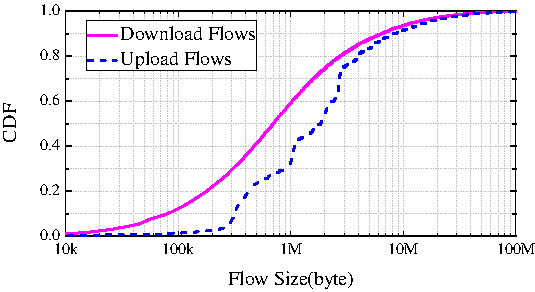
\includegraphics[width=\linewidth]{flow-size}
%	\caption{Upload and download flows size.}
%	\label{fig:flow-size}
%	\termspace
%\end{figure}

Figure~\ref{fig:flow-rate} shows the upload and download flows' rate. From the figure we can see that the upload flows' rate is smaller than the download flow. Two reasons account for it. First, for most network, the bandwidth of the upload is smaller than the download. For example, the upload bandwidth of ADSL(Asymetric Digital Subscriber Loop) is 640Kbps while the download bandwidth is 6-8Mbps~\cite{wei2008classification}. Second, as download flows is fetched from the storage server without waiting while the upload flows can only send data when cameras produce video data. 
%\begin{figure}[ht]
%	\centering
%	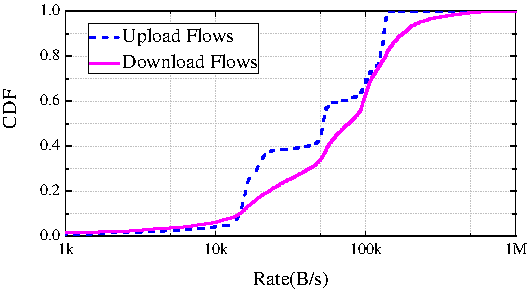
\includegraphics[width=\linewidth]{rate}
%	\caption{The rate of upload and download flow.}
%	\label{fig:flow-rate}
%	\termspace
%\end{figure}
